% ----------------------------------------------------------------------
%  Před psaním se důkladně seznamte s Pravidly pro vypracování protokolu!
% ----------------------------------------------------------------------

% ----------------------------------------------------------------------
%  Pracovní úkoly - opište přímo ze zadání
% ----------------------------------------------------------------------
%\section{Pracovní úkoly}

%\begin{enumerate}
%\item ...

%\end{enumerate}

% ----------------------------------------------------------------------
%  Použité pomůcky
% ----------------------------------------------------------------------

%\newpage


%\begin{figure}[H]
%	\centering
%	\includegraphics[scale = 0.5]{img/schema_regulovane_soustavy.png} 
%	\caption{Schéma regulované soustavy.} 
%	\label{fig:schema_reg}
%\end{figure}	

%\begin{figure}[H] 
%	\centering
%	\includegraphics[scale = 0.7]{img/schema_PID_regulatoru.png} 
%	\caption{Schéma PID regulátoru.} 
%	\label{fig:schema_PID}
%\end{figure}		
		

% ----------------------------------------------------------------------
%  Teoretický úvod - vlastními slovy stručne popište fyzikální podstatu měření a uveďte základní vztahy použité ve vypracování
% ----------------------------------------------------------------------
%\section{Teoretický úvod}	

% ----------------------------------------------------------------------
%  Postup měření - vlastními slovy popište postup měření tak, aby bylo vaše měření reprodukovatelné 
% ----------------------------------------------------------------------
%\section{Postup měření}
			
% ----------------------------------------------------------------------
%  Naměřené hodnoty a samotné vypracování úkolu
% ----------------------------------------------------------------------	
			
\section{Vypracování}
\subsection{Charakteristika laseru v režimu volné generace}
Závislosti výstupní energie $E$ a účinnosti $\eta$ na budící energii $E_\mathrm{b}$ pro zrcadla M337, M327 a křemenné sklo jsou uvedeny v Tab.~\ref{tab:ucinnost_zrcadla} a v grafech na Obr.~\ref{fig:ucinnost_M337},~\ref{fig:ucinnost_kremenne_sklo},~\ref{fig:ucinnost_M327}.

Závislost délky impulsu $\tau_\mathrm{FR}$, a středního výkonu $P_\mathrm{str}$ na budící energii $E_\mathrm{b}$ pro pro optimální zrcadlo (M327) je uvedena v Tab.~\ref{tab:optimalni_zrcadlo} a vykreslena na Obr.~\ref{fig:optimalni_zrcadlo}.\\
Hustota energie při maximální energii $\rho_\mathrm{max}=8,73\unit{J\cdot cm^{-2}}$ \\
Obrázky časových průběhů záření jsou na Obr.~\ref{fig:cas_1},~\ref{fig:cas_2}~a~\ref{fig:cas_3}.

\begin{table}[!hbt]
\centering
	\begin{tabular}{|c|c|c||c|c|c||c|c|c|}
		\hline
		\multicolumn{3}{|c||}{M337}					&	\multicolumn{3}{c||}{křemenné sklo}					&	\multicolumn{3}{c|}{M327}					\\ \hline
$\tabh{E_\mathrm{b}}{J}$	&	\tabh{E}{J}	&	\tabh{\eta}{\%}	&	$\tabh{E_\mathrm{b}}{J}$	&	\tabh{E}{J}	&	\tabh{\eta}{\%}	&	$\tabh{E_\mathrm{b}}{J}$	&	\tabh{E}{J}	&	\tabh{\eta}{\%}	\\ \hline \hline
13,62	&	0,00	&	0,00	&	15,21	&	0,00	&	0,00	&	13,76	&	0,00	&	0,00	\\ \hline
14,14	&	0,02	&	0,16	&	16,89	&	0,02	&	0,11	&	14,14	&	0,02	&	0,15	\\ \hline
15,21	&	0,04	&	0,29	&	19,27	&	0,08	&	0,40	&	15,21	&	0,07	&	0,45	\\ \hline
16,89	&	0,07	&	0,39	&	22,37	&	0,15	&	0,68	&	16,89	&	0,13	&	0,74	\\ \hline
19,27	&	0,10	&	0,50	&	26,52	&	0,24	&	0,89	&	19,27	&	0,19	&	1,01	\\ \hline
22,37	&	0,14	&	0,60	&	31,70	&	0,35	&	1,10	&	22,37	&	0,27	&	1,21	\\ \hline
26,52	&	0,19	&	0,71	&	34,22	&	0,39	&	1,14	&	26,52	&	0,34	&	1,30	\\ \hline
31,70	&	0,25	&	0,78	&	38,32	&	0,47	&	1,24	&	31,70	&	0,45	&	1,41	\\ \hline
38,32	&	0,33	&	0,87	&	42,90	&	0,56	&	1,30	&	38,32	&	0,58	&	1,51	\\ \hline
46,38	&	0,40	&	0,85	&	48,16	&	0,66	&	1,37	&	46,38	&	0,72	&	1,55	\\ \hline
56,25	&	0,51	&	0,90	&	56,25	&	0,81	&	1,44	&	56,25	&	0,89	&	1,58	\\ \hline

	\end{tabular}
	\caption{Závislosti výstupní energie $E$ a účinnosti $\eta$ na budící energii $E_\mathrm{b}$ pro zrcadla M337, M327 a křemenné sklo.}
	\label{tab:ucinnost_zrcadla}
\end{table}

\begin{figure}[H] 
	\centering
	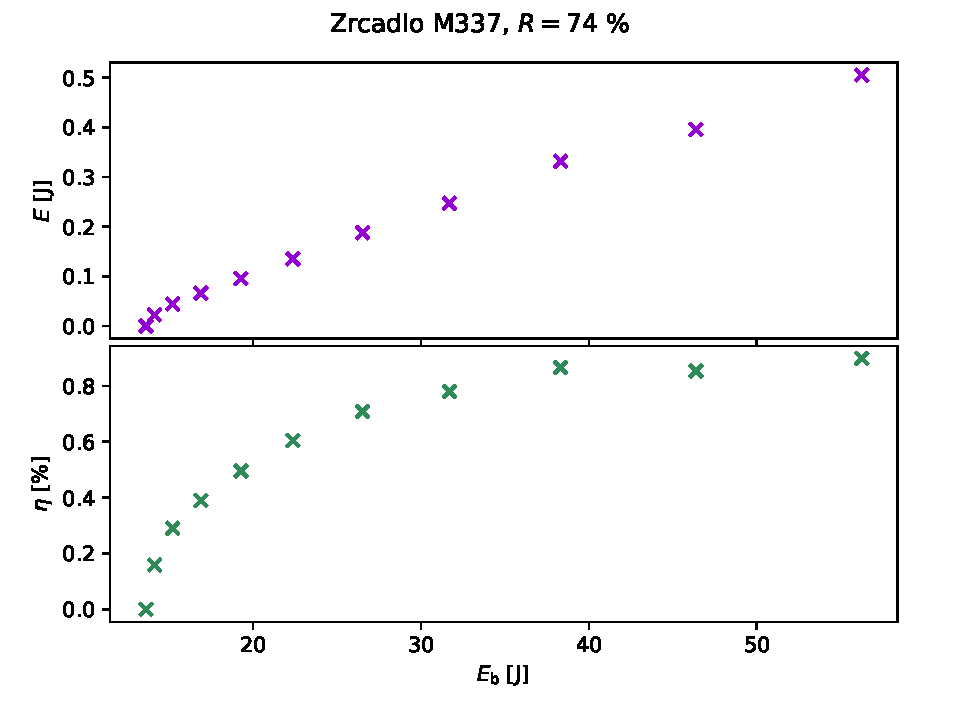
\includegraphics[scale = 0.7]{img/zrcadlo_M337.pdf} 
	\caption{Závislost výstupní energie $E$ a účinnosti $\eta$ na budící energii $E_\mathrm{b}$ pro zrcadlo M337.} 
	\label{fig:ucinnost_M337}
\end{figure}


\begin{figure}[H] 
	\centering
	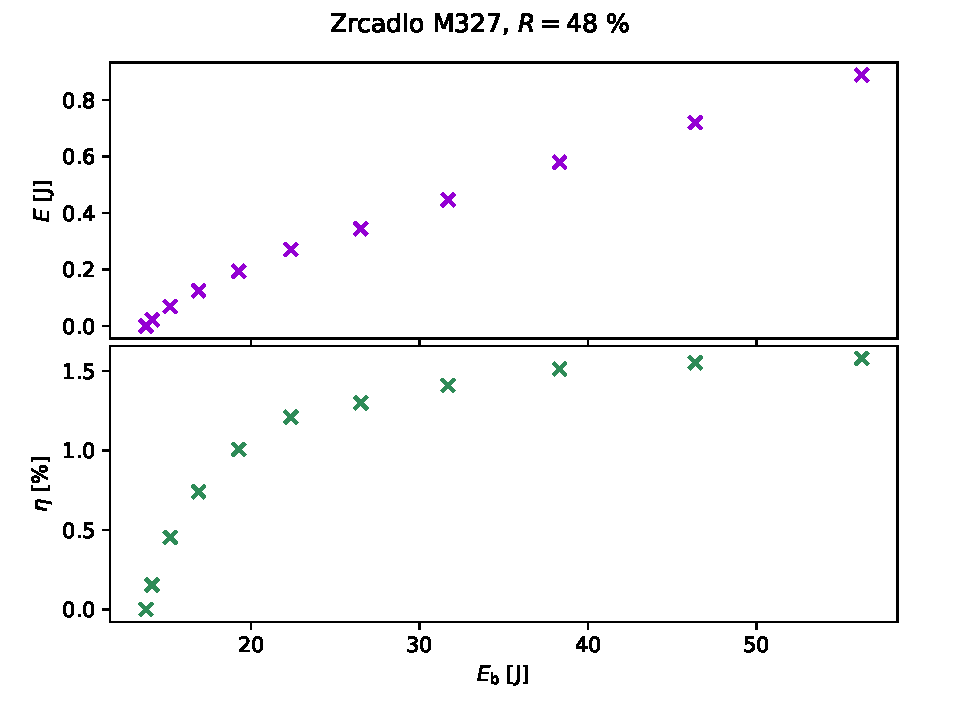
\includegraphics[scale = 0.7]{img/zrcadlo_M327.pdf} 
	\caption{Závislost výstupní energie $E$ a účinnosti $\eta$ na budící energii $E_\mathrm{b}$ pro zrcadlo M327.} 
	\label{fig:ucinnost_M327}
\end{figure}


\begin{figure}[H] 
	\centering
	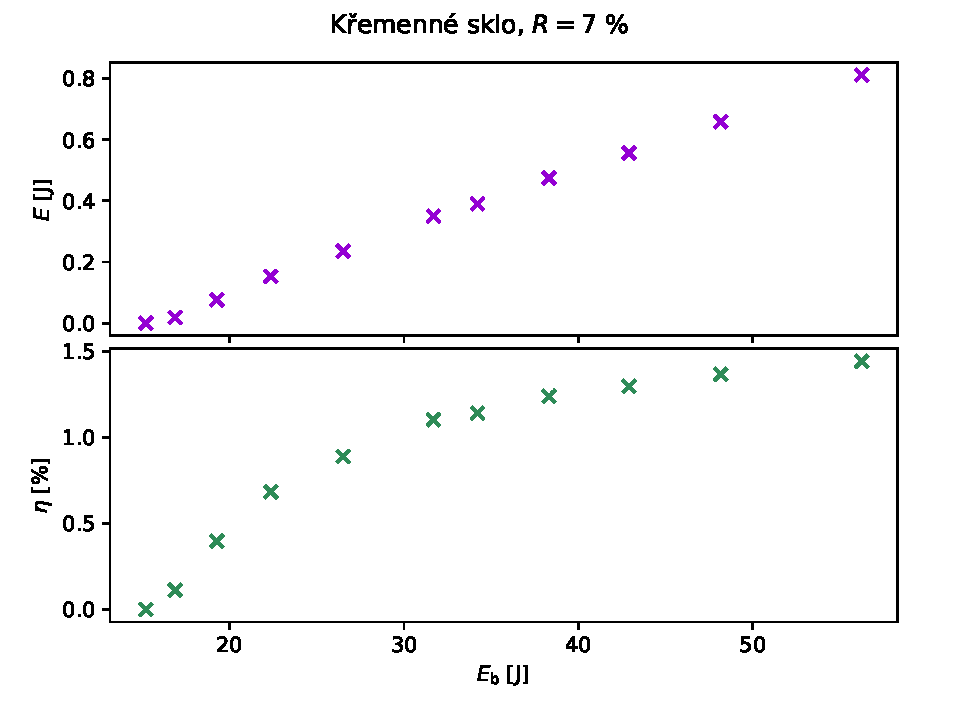
\includegraphics[scale = 0.7]{img/zrcadlo_kremenne_sklo.pdf} 
	\caption{Závislost výstupní energie $E$ a účinnosti $\eta$ na budící energii $E_\mathrm{b}$ pro zrcadlo z křemenného skla.} 
	\label{fig:ucinnost_kremenne_sklo}
\end{figure}


\begin{table}[!hbt]
\centering
	\begin{tabular}{|c||c|c|}
		\hline
$\tabh{E_\mathrm{b}}{J}$ & \tabh{\tau}{\mu s} & $\tabh{P_\mathrm{str}}{kW}$ \\ \hline \hline
13,76 & 63 & 0 \\ \hline
31,70 & 308 & 1,450 \\ \hline
56,25 & 83 & 10,674 \\ \hline
	\end{tabular}
	\caption{Závislost délky impulsu $\tau_\mathrm{FR}$, a středního výkonu $P_\mathrm{str}$ na budící energii $E_\mathrm{b}$ pro zrcadlo M327.}
	\label{tab:optimalni_zrcadlo}
\end{table}

\begin{figure}[H] 
	\centering
	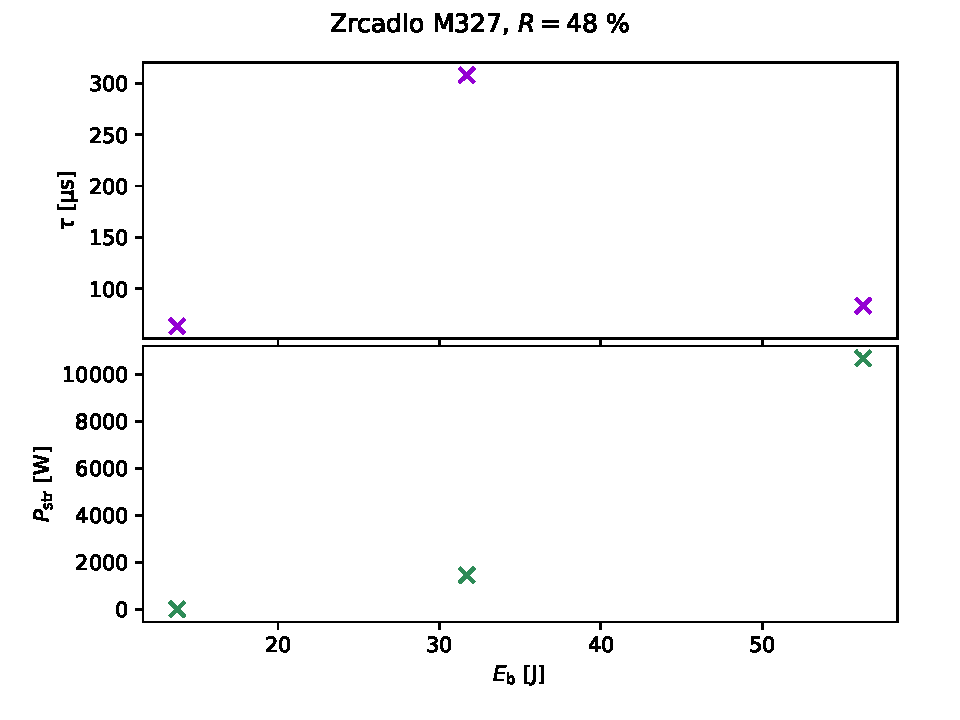
\includegraphics[scale = 0.7]{img/optimalni_zrcadlo.pdf} 
	\caption{Závislost délky impulsu $\tau_\mathrm{FR}$, a středního výkonu $P_\mathrm{str}$ na budící energii $E_\mathrm{b}$ pro zrcadlo M327.} 
	\label{fig:optimalni_zrcadlo}
\end{figure}

\begin{figure}[H] 
	\centering
	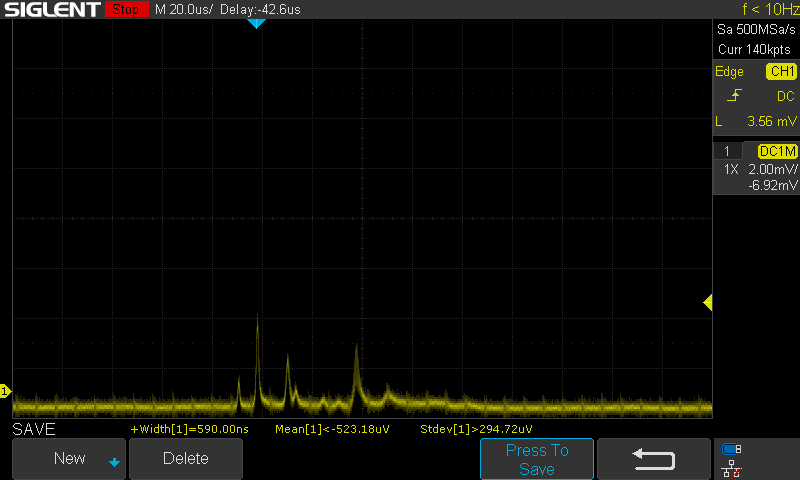
\includegraphics[scale = 0.5]{img/SDS00002.png} 
	\caption{Časový průbeh impulsu pro $E_\mathrm{b}$=13,76 J} 
	\label{fig:cas_1}
\end{figure}

\begin{figure}[H] 
	\centering
	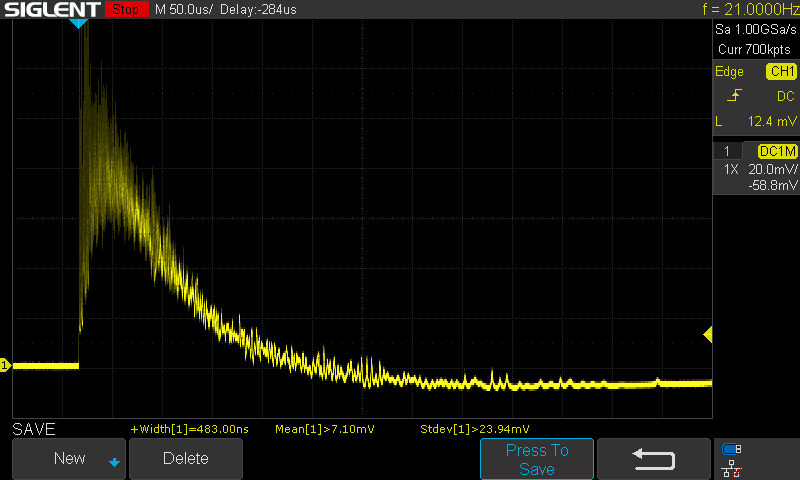
\includegraphics[scale = 0.5]{img/SDS00004.png} 
	\caption{Časový průbeh impulsu pro $E_\mathrm{b}$=31,70 J} 
	\label{fig:cas_2}
\end{figure}

\begin{figure}[H] 
	\centering
	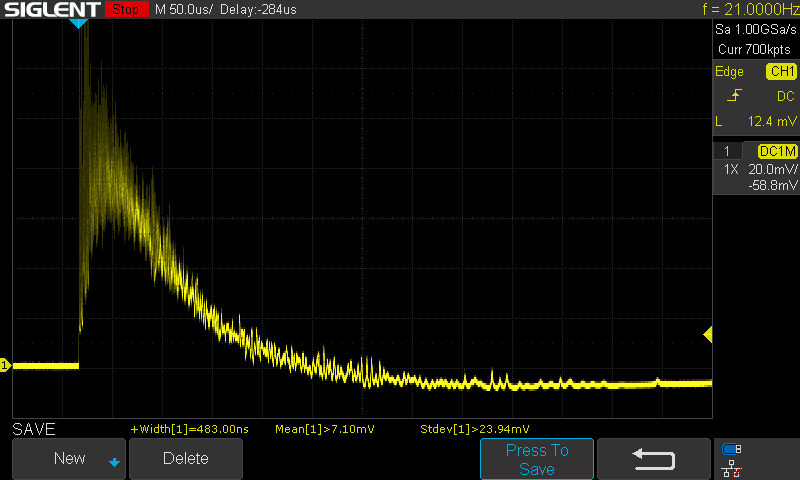
\includegraphics[scale = 0.5]{img/SDS00004.png} 
	\caption{Časový průbeh impulsu pro $E_\mathrm{b}$=65,25 J} 
	\label{fig:cas_3}
\end{figure}


\subsection{Zesilování impulsů}
Závislost zesílení impulsu $G$ na budící energii $E_\mathrm{b}$ laserového oscilátoru pro optimální zrcadlo (M327) je na Obr.\ref{fig:zasileni}.
\begin{figure}[H] 
	\centering
	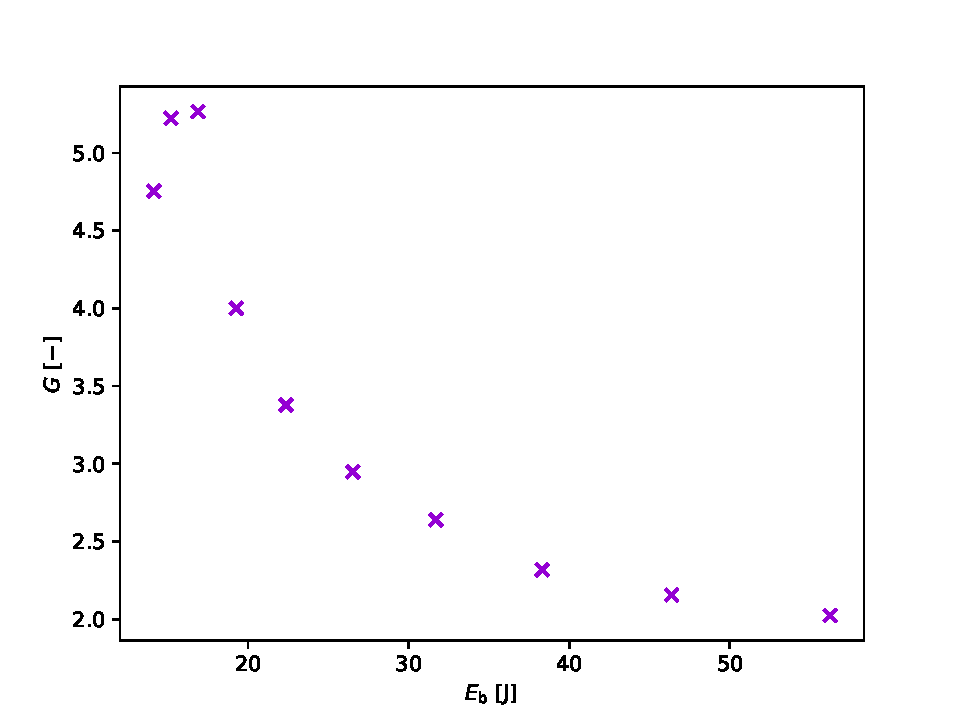
\includegraphics[scale = 0.7]{img/zesileni.pdf} 
	\caption{Závislost zesílení impulsu $G$ na budící energii $E_\mathrm{b}$ laserového oscilátoru pro zrcadlo M327.} 
	\label{fig:zasileni}
\end{figure}

\subsection{Q-spínaný režim}
Výsledky měření délky $\tau$, energie $E$, špičkového výkonu $P_\mathrm{peak}$ a plošné hustoty energie $\rho$ Q-spínaných impulsů jsou v Tab.~\ref{tab:q_spinani}. \\
Hustota energie v Q-spínaném režimu je oproti režimu volné generace přibližně $100\times$ vyšší.
Záznam časového vývoje z osciloskopu

\begin{table}[!hbt]
\centering
	\begin{tabular}{|c|c|c|c|c|}
		\hline
	&	\tabh{\tau}{ns}	&	\tabh{E}{mJ}	&	$\tabh{P_\mathrm{peak}}{kW}$	&	\tabh{\rho}{J\cdot cm^{-2}}	\\ \hline	\hline
	&	25	&	51	&	2075	&	773	\\ \hline	
	&	24	&	51	&	2145	&	773	\\ \hline	
	&	27	&	54	&	2042	&	819	\\ \hline	
	&	30	&	65	&	2154	&	981	\\ \hline	
	&	26	&	52	&	2000	&	784	\\ \hline	
	&	22	&	48	&	2245	&	734	\\ \hline	
	&	28	&	67	&	2362	&	1008	\\ \hline	
	&	26	&	45	&	1761	&	680	\\ \hline	
	&	25	&	66	&	2612	&	1005	\\ \hline	
	&	25	&	52	&	2048	&	784	\\ \hline	\hline
Průměr	&	26	&	55	&	2144	&	834	\\ \hline	
Odchylka	&	2	&	7	&	216	&	113	\\ \hline	


	\end{tabular}
	\caption{Výsledky měření délky $\tau$, energie $E$, špičkového výkonu $P_\mathrm{peak}$ a plošné hustoty energie $\rho$ Q-spínaných impulsů.}
	\label{tab:q_spinani}
\end{table}


\begin{figure}[H] 
	\centering
	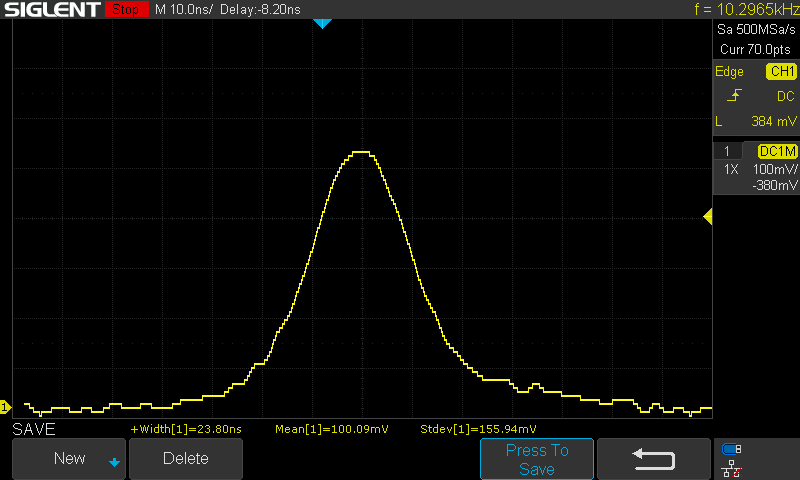
\includegraphics[scale = 0.5]{img/SDS00008.png} 
	\caption{Záznam časového vývoje z osciloskopu pro Q-spínaný puls.}
	\label{fig:cas_3}
\end{figure}
% ----------------------------------------------------------------------
%  Diskuse - obsahuje komentář k jednotlivým výsledkům, porovnání s očekáváním/tabulkovými hodnotami, zdroje především systematických chyb měření, návrh na zlepšení výsledků,...
% ----------------------------------------------------------------------			
%\section{Diskuse}			

% ----------------------------------------------------------------------
%  Závěr - stručně a jasně shrnout splněné cíle měření, úkoly a výsledky měření
% ----------------------------------------------------------------------
			
%\section{Závěr}



